\subsection{Kasseapperat}
I de følgende afsnit vil der kunne læses om unittests for \gls{KA}.\\\\

\textbf{Introduktion}\\
\gls{KA} har været testet itterativt over udviklingsperioden. Det har bidgraget
væsentligt med at finde små fejl, som ellers var gået igennem. I de nedenstående afsnit vil der
kunne læses om hvordan der er testet, med hvilke frameworks og mere konkrete tal.\\

\textbf{Testdetaljer}\\
I administrationssystemet er der en total testcoverage på \textit{72} procent af testbare klasser\footnote{GUI, eksterne klasser, XML mv er \textit{ikke} en del af testbare klasser.}. Dette summerer sig op til 51 unittests, som er fordelt over ViewModels, Business Logic og Data Access. Testene er lavet
vha. NUnit~\cite{NUnit} og NSubstitute~\cite{NSubstitute} og coverage analyse er foretaget med dotCover~\cite{dotCover}.

\begin{figure}[H]
	\centering
	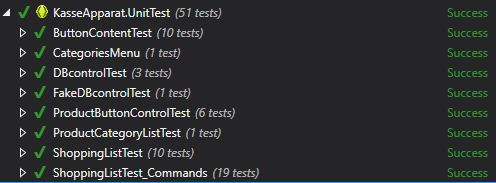
\includegraphics[width=0.90\textwidth]{Test/Images/Frontend/UnitTests}
	\caption{Unit Tests for Kasseapparat}
	\label{fig:UTKA}
\end{figure}

\begin{figure}[H]
	\centering
	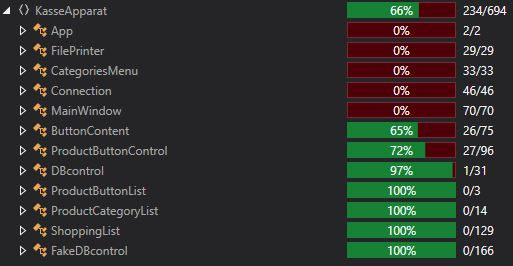
\includegraphics[width=0.90\textwidth]{Test/Images/Frontend/UnitTestCover}
	\caption{Unit Tests Coverage for Kasseapparat}
	\label{fig:UTCKA}
\end{figure}

\textbf{Beskrivelse af tests}\\
I \gls{KA} har der været stor fokus på at teste ShoppingList, da denne har stort ansvar i form af at håndtere vare i et salg. ShoppingList er især blevet testet med henblik på dennes commands. Disse er blevet testet med BVA\footnote{Boundary Value Analysis} omkring 0, for at sikre at disse kun kan ekseveres når der er produkter på ShoppingListen, samt om de udføre korrekte funktionalitet, når de eksekveres.\\
...